% little trick to replace lib.tex by this
\renewcommand{\doctitle}[1]{
	\chapter{#1}
}
\renewcommand{\biblio}[1]{}
\doctitle{LELEC1101 - Problème 1}

On s'intéresse ici à un signal triangulaire $u(t)$
périodique, symétrique, de période $T$ et de valeurs 
minimales et maximales $V_{\text{min}}$ et $V_{\text{max}}$
respectivement. On peut décomposer cette fonction
en série de Fourier
\[ u(t) = A_0 + \sum_{k=1}^{\infty} A_k\cos(k\omega t)
+ \sum_{k=1}^{\infty} B_k\sin(k\omega t). \]
où $\omega = \frac{2\pi}{T}$ est la pulsation angulaire.
La composante constante $A_0$ et les coefficients $A_k$
et $B_k$ sont donnés par 
\[ A_0 = \frac{1}{T} \int_0^T u(t)\dif t,\]
\[ A_k = \frac{2}{T} \int_0^T u(t)\cos(k\omega t)\dif t,\]
\[ B_k = \frac{2}{T} \int_0^T u(t)\sin(k\omega t)\dif t.\]

\section{Question 1}
Etablissons dans un premier temps la série de Fourier
dans le cas particulier où le signal triangulaire
est symétrique (i.e. $u(t) = u(-t)$) et centrée autour
de l'axe de $t$. Dans ce cas particulier, on a $A_0 = 0$
et $B_k = 0$. On peut donc réecrire la décomposition
en série de Fourier 
\[ u(t) = \sum_{k=1}^{\infty} A_k\cos(k\omega t).\]
Calculons maintenant les coefficients
\[ A_k = \frac{2}{T} \int_0^T u(t)\cos(k\omega t)\dif t.\]
Pour cela, on décompose $u(t)$ sur l'intervalle $[0,T]$
en deux parties
\[ u(t) =
	\left\{
		\begin{array}{rl}
			V_{\text{max}} - \frac{2(V_{\text{max}-V_{\text{min}}})}{T}t 	
			&\text{ pour } t \in [0,\frac{T}{2}]  \\
			2V_{\text{min}} + \frac{2(V_{\text{max}-V_{\text{min}}})}{T}t 
			&\text{ pour }t \in [\frac{T}{2},T] 
		\end{array}
	\right.
\]
On peut alors facilement décomposer l'intégrale en deux
parties. On trouve donc\footnote{Les détails
de calculs sont omis ici.}
\[ A_k = \frac{2}{\pi^2k^2}(V_{\text{max}}-V_{\text{min}})
(1 - (-1)^k).\]
où $\cos(k\pi)$ a été remplacé par $(-1)^k$.
On a finalement
\[ u(t) = \frac{2}{\pi^2}(V_{\text{max}}-V_{\text{min}})
\sum_{k=1}^{\infty} \frac{1}{k^2}(1 - (-1)^k)\cos(k\omega t).\]
On peut ensuite vérifier, à l'aide de \matlab,
que cette décomposition en série de Fourier
converge effectivement vers le signal triangulaire.
La figure \ref{fig:q1-fourier-10} est la décomposition
en série de Fourier pour $k = 1\cdots10$ pour 
$T = \unit{1}{\second}$ et $V_{\text{max}} = 
-V_{\text{min}} = \unit{5}{\volt}$.

\begin{figure}[ht]
	\centering
	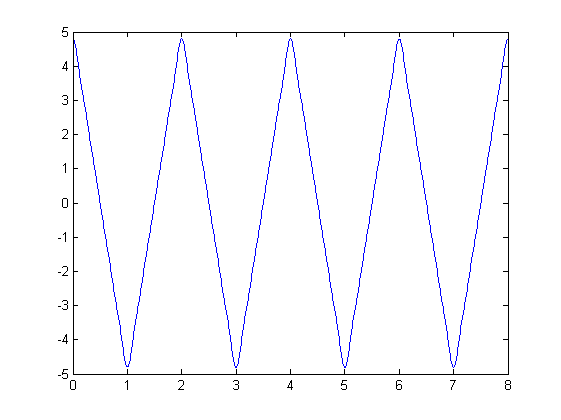
\includegraphics[scale=0.75]{img/q1-fourier-10.png}
	\caption{Décomposition en série de Fourier pour $k=1\cdots10$.}
	\label{fig:q1-fourier-10}
\end{figure}

\end{document}
